\def\mytitle{TRIANGLES}
\documentclass[10pt,a4paper]{article}
\def\inputGnumericTable{}
\usepackage[margin=0.3in]{geometry}
   \usepackage[latin1]{inputenc}
   \usepackage{fullpage}
	\usepackage{color}
	\usepackage{array}
   \usepackage{longtable}
     \usepackage{calc}
       \usepackage{multirow}
       \usepackage{hhline}
       \usepackage{ifthen}
\usepackage{gensymb}       
\usepackage{graphicx}
\graphicspath{{./images/}}
\usepackage[colorlinks,linkcolor={black},citecolor={blue!80!black},urlcolor={blue!80!black}]{hyperref}
\usepackage[parfill]{parskip}
\usepackage{lmodern}
\usepackage{tikz}
\usepackage{physics}
\usepackage{tabularx}
\usepackage{enumitem}
\usetikzlibrary{calc}
\usepackage{amsmath}
\usepackage{amssymb}
\renewcommand*\familydefault{\sfdefault}
\usepackage{watermark}
\usepackage{lipsum}
\usepackage{xcolor}
\usepackage{listings}
\usepackage{float}
\usepackage{titlesec}
\providecommand{\mtx}[1]{\mathbf{#1}}
\titlespacing{\subsection}{1pt}{\parskip}{3pt}
\titlespacing{\subsubsection}{0pt}{\parskip}{-\parskip}
\titlespacing{\paragraph}{0pt}{\parskip}{\parskip}


\newcommand{\myvec}[1]{\ensuremath{\begin{pmatrix}#1\end{pmatrix}}}
\let\vec\mathbf
\lstset{
frame=single, 
breaklines=true,
columns=fullflexible
}
\title{\mytitle}
\begin{document}
\begin{center}
\textbf\large{ STRAIGHT LINES}\\
\textbf\large{Exercise 7.1}
\end{center}

\tableofcontents
\section{Problem}
Q3. AD and BC are equal perpendiculars to a line segment. Show that CD bisects AB.
\begin{figure}[!h]
	\begin{center}
		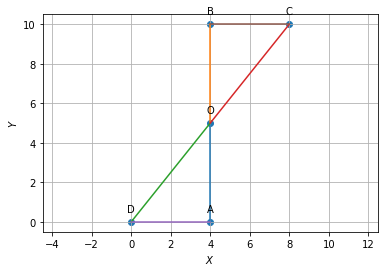
\includegraphics[width=5in]{./figs/figure.png}
	\end{center}
\caption{}
\label{figure}
\end{figure}
\pagebreak
\section{Construction}
The input parameters are the lengths a and c.\\
{
\setlength\extrarowheight{2pt}
\begin{tabular}{|c|c|c|}
	\hline
	\textbf{Symbol}&\textbf{Value}&\textbf{Description}\\
	\hline
	a&4&$\vec{A}\vec{D}=\vec{B}\vec{C}$\\
	\hline
	c&3&$\vec{O}\vec{A}=\vec{O}\vec{B}$\\
	\hline
	$\theta$&arctan$\myvec{\frac{c}{a}}$&$\angle{D}=\angle{C}$\\
	\hline
	O&$\sqrt{a^2+c^2}%
	\begin{pmatrix}
		cos\theta\\
		sin\theta\\
	\end{pmatrix}$%
	&Point O\\
	\hline
\end{tabular}
}
\section{Solution}
\textbf{Given:}
\begin{align}
    AD=BC\\
    \angle{CBO}=\angle{DAO}
\end{align}
\textbf{To prove :}
\begin{align}
    \angle{ODA}=\angle{OCB}
\end{align}
\textbf{Proof}\\
The directional vectors are:
\begin{align}
    \vec{m_1}=\Vec{O}-\Vec{D}\\
    \vec{m_2}=\Vec{D}-\Vec{A}
\end{align}
The Normal vectors are:
\begin{align}
    \vec{n_1}=\Vec{O}-\Vec{C}\\
    \vec{n_2}=\Vec{C}-\Vec{B}\\
\end{align}
\begin{align}
	\theta_1 =cos^{-1}\myvec{\frac{\vec{m_1}^T\vec{m_2}}{\norm{\vec{m_1}}\norm{\vec{m_2}}}}\\
	\theta_2 =\cos^{-1}\myvec{\frac{\vec{n_1}^T\vec{n_2}}{\norm{\vec{n_1}}\norm{\vec{n_2}}}}
\end{align}
If $\theta_1 = \theta_2$
\begin{align}
    \triangle{OBC} \cong \triangle{OAD}\\
    OA = OB
\end{align}
\end{document}
